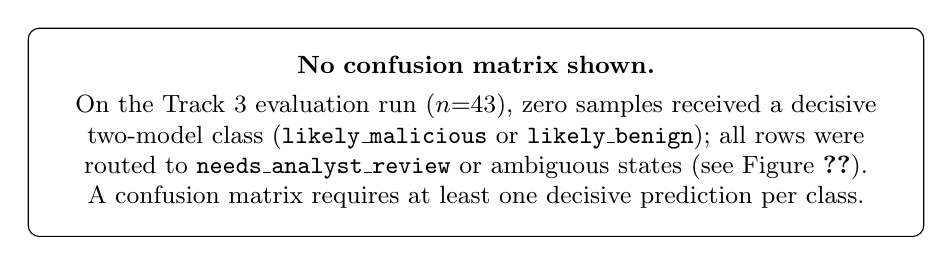
\begin{tikzpicture}
\node[
  draw,
  rounded corners,
  align=center,
  inner sep=10pt,
  text width=0.88\linewidth,
  font=\small
] {
  \textbf{No confusion matrix shown.}\\[0.35em]
  On the Track~3 evaluation run ($n{=}43$), zero samples received a decisive two-model class
  (\texttt{likely\_malicious} or \texttt{likely\_benign}); all rows were routed to
  \texttt{needs\_analyst\_review} or ambiguous states (see Figure~\ref{fig:two_model_triage}).
  A confusion matrix requires at least one decisive prediction per class.
};
\end{tikzpicture}
